% PROPOSED PEDAGOGICAL FIGURES FOR TINYTORCH PAPER
% Generated: 2025-11-17
% Status: Draft - Ready for Review and Integration

\documentclass{article}
\usepackage{tikz}
\usetikzlibrary{shapes,arrows,positioning,decorations.pathreplacing,calc}
\usepackage{geometry}
\geometry{margin=1in}
\usepackage{xcolor}

% Define colors matching paper
\definecolor{accentcolor}{RGB}{255,87,34}
\definecolor{dormantgray}{RGB}{200,200,200}
\definecolor{activeorange}{RGB}{255,152,0}

\begin{document}

\section*{Proposed Pedagogical Figures for TinyTorch Paper}

% ============================================================
% FIGURE A: PROGRESSIVE DISCLOSURE TIMELINE
% ============================================================
\subsection*{Figure A: Progressive Disclosure Timeline (HIGHEST PRIORITY)}
\textbf{Location:} Section 3.1 (Progressive Disclosure), after Listing 2\\
\textbf{Pedagogical Value:} Visualizes the paper's most novel contribution - how Tensor capabilities evolve across modules while maintaining single mental model.

\begin{figure}[h]
\centering
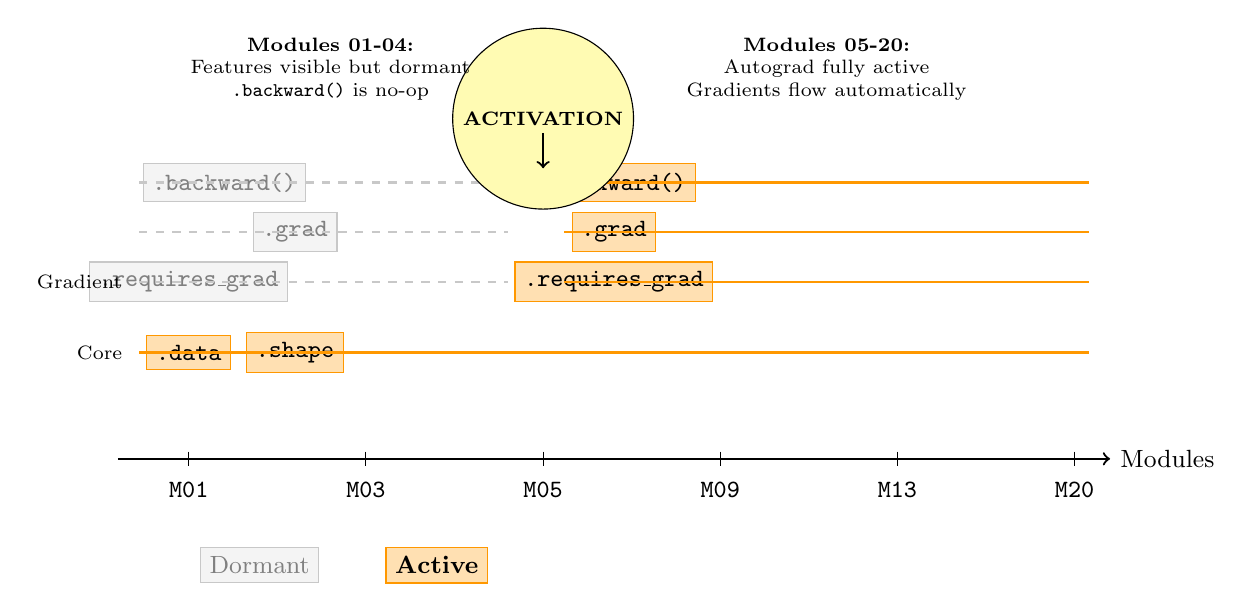
\begin{tikzpicture}[
    scale=0.9,
    every node/.style={font=\small},
    module/.style={rectangle, draw, fill=blue!20, minimum width=1.2cm, minimum height=0.8cm},
    dormant/.style={rectangle, draw=dormantgray, fill=dormantgray!20, text=gray},
    active/.style={rectangle, draw=activeorange, fill=activeorange!30, text=black, font=\small\bfseries}
]

% Timeline axis
\draw[thick, ->] (0,0) -- (14,0) node[right] {Modules};

% Module markers
\foreach \x/\label in {1/01, 3.5/03, 6/05, 8.5/09, 11/13, 13.5/20} {
    \draw (\x, 0.1) -- (\x, -0.1);
    \node[below] at (\x, -0.2) {\texttt{M\label}};
}

% Feature layers - stacked above timeline
% Layer 1: Basic Tensor (always present)
\node[active] at (1, 1.5) {\texttt{.data}};
\node[active] at (2.5, 1.5) {\texttt{.shape}};
\draw[activeorange, thick] (0.3, 1.5) -- (13.7, 1.5);
\node[left, font=\scriptsize] at (0.2, 1.5) {Core};

% Layer 2: Dormant until Module 05
\node[dormant] at (1, 2.5) {\texttt{.requires\_grad}};
\draw[dormantgray, thick, dashed] (0.3, 2.5) -- (5.5, 2.5);
\node[active] at (7, 2.5) {\texttt{.requires\_grad}};
\draw[activeorange, thick] (6.3, 2.5) -- (13.7, 2.5);
\node[left, font=\scriptsize] at (0.2, 2.5) {Gradient};

\node[dormant] at (2.5, 3.2) {\texttt{.grad}};
\draw[dormantgray, thick, dashed] (0.3, 3.2) -- (5.5, 3.2);
\node[active] at (7, 3.2) {\texttt{.grad}};
\draw[activeorange, thick] (6.3, 3.2) -- (13.7, 3.2);

\node[dormant] at (1.5, 3.9) {\texttt{.backward()}};
\draw[dormantgray, thick, dashed] (0.3, 3.9) -- (5.5, 3.9);
\node[active] at (7, 3.9) {\texttt{.backward()}};
\draw[activeorange, thick] (6.3, 3.9) -- (13.7, 3.9);

% Activation marker at Module 05
\node[draw, fill=yellow!30, circle, font=\scriptsize\bfseries] at (6, 4.8) {ACTIVATION};
\draw[thick, ->] (6, 4.6) -- (6, 4.1);

% Annotations
\node[align=center, font=\scriptsize] at (3, 5.5) {
    \textbf{Modules 01-04:}\\
    Features visible but dormant\\
    \texttt{.backward()} is no-op
};

\node[align=center, font=\scriptsize] at (10, 5.5) {
    \textbf{Modules 05-20:}\\
    Autograd fully active\\
    Gradients flow automatically
};

% Legend
\node[dormant, minimum width=1cm] at (2, -1.5) {Dormant};
\node[active, minimum width=1cm] at (4.5, -1.5) {Active};

\end{tikzpicture}
\caption{Progressive disclosure of \texttt{Tensor} capabilities across modules. Gradient-related features (\texttt{.requires\_grad}, \texttt{.grad}, \texttt{.backward()}) exist from Module 01 but remain dormant (gray, dashed) until Module 05 activates them via monkey-patching (orange, solid). Students work with a single \texttt{Tensor} interface throughout, but capabilities expand progressively. This manages cognitive load while maintaining conceptual unity.}
\label{fig:progressive-timeline}
\end{figure}

\clearpage

% ============================================================
% FIGURE B: MEMORY HIERARCHY BREAKDOWN
% ============================================================
\subsection*{Figure B: Memory Hierarchy Breakdown (HIGH PRIORITY)}
\textbf{Location:} Section 4.1 (Memory Profiling), after Table 1\\
\textbf{Pedagogical Value:} Clarifies that "Adam uses 3× parameter memory" refers to optimizer state, while activations typically dominate total memory. Visual makes this concrete.

\begin{figure}[h]
\centering
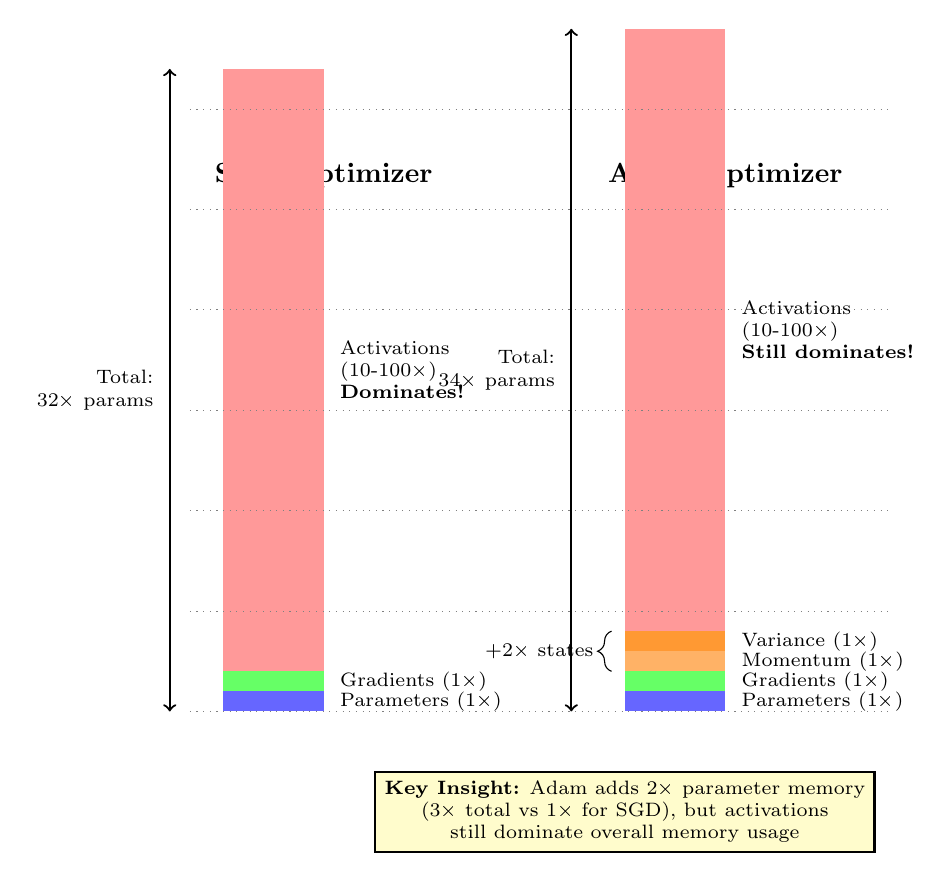
\begin{tikzpicture}[
    scale=0.85,
    every node/.style={font=\small}
]

% Define bar widths and positions
\def\barwidth{1.5}
\def\unitheight{0.3}

% SGD Memory Breakdown (Left)
\node[font=\normalsize\bfseries] at (2, 8) {SGD Optimizer};

% Parameters (1x)
\fill[blue!60] (0.5, 0) rectangle +({\barwidth}, {1*\unitheight});
\node[right, font=\scriptsize] at (2.1, {0.5*\unitheight}) {Parameters (1×)};

% Gradients (1x)
\fill[green!60] (0.5, {1*\unitheight}) rectangle +({\barwidth}, {1*\unitheight});
\node[right, font=\scriptsize] at (2.1, {1.5*\unitheight}) {Gradients (1×)};

% Activations (10-100x)
\fill[red!40] (0.5, {2*\unitheight}) rectangle +({\barwidth}, {30*\unitheight});
\node[right, font=\scriptsize, align=left] at (2.1, {17*\unitheight}) {
    Activations\\(10-100×)\\
    \textbf{Dominates!}
};

% Total annotation
\draw[thick, <->] (-0.3, 0) -- (-0.3, {32*\unitheight});
\node[left, font=\scriptsize, align=right] at (-0.4, {16*\unitheight}) {
    Total:\\32× params
};

% Adam Memory Breakdown (Right)
\node[font=\normalsize\bfseries] at (8, 8) {Adam Optimizer};

% Parameters (1x)
\fill[blue!60] (6.5, 0) rectangle +({\barwidth}, {1*\unitheight});
\node[right, font=\scriptsize] at (8.1, {0.5*\unitheight}) {Parameters (1×)};

% Gradients (1x)
\fill[green!60] (6.5, {1*\unitheight}) rectangle +({\barwidth}, {1*\unitheight});
\node[right, font=\scriptsize] at (8.1, {1.5*\unitheight}) {Gradients (1×)};

% Adam states: momentum (1x)
\fill[orange!60] (6.5, {2*\unitheight}) rectangle +({\barwidth}, {1*\unitheight});
\node[right, font=\scriptsize] at (8.1, {2.5*\unitheight}) {Momentum (1×)};

% Adam states: variance (1x)
\fill[orange!80] (6.5, {3*\unitheight}) rectangle +({\barwidth}, {1*\unitheight});
\node[right, font=\scriptsize] at (8.1, {3.5*\unitheight}) {Variance (1×)};

% Brace for optimizer states
\draw[decorate, decoration={brace, amplitude=5pt}]
    (6.3, {2*\unitheight}) -- (6.3, {4*\unitheight})
    node[midway, left, xshift=-3pt, font=\scriptsize] {+2× states};

% Activations (10-100x) - same as SGD
\fill[red!40] (6.5, {4*\unitheight}) rectangle +({\barwidth}, {30*\unitheight});
\node[right, font=\scriptsize, align=left] at (8.1, {19*\unitheight}) {
    Activations\\(10-100×)\\
    \textbf{Still dominates!}
};

% Total annotation
\draw[thick, <->] (5.7, 0) -- (5.7, {34*\unitheight});
\node[left, font=\scriptsize, align=right] at (5.6, {17*\unitheight}) {
    Total:\\34× params
};

% Key insight box
\node[draw, thick, fill=yellow!20, align=center, font=\scriptsize] at (6.5, -1.5) {
    \textbf{Key Insight:} Adam adds 2× parameter memory\\
    (3× total vs 1× for SGD), but activations\\
    still dominate overall memory usage
};

% Grid lines for easier reading
\foreach \y in {0,5,10,15,20,25,30} {
    \draw[dotted, gray] (0, {\y*\unitheight}) -- (10.5, {\y*\unitheight});
}

\end{tikzpicture}
\caption{Memory hierarchy breakdown comparing SGD and Adam optimizers. While Adam requires 3× parameter memory (parameters + gradients + momentum + variance) compared to SGD's 2× (parameters + gradients), activation memory typically dominates total memory consumption by 10-100×. This visualization clarifies that optimizer choice affects parameter memory overhead, but activation memory remains the primary concern for most models. Students learn to calculate each component from Module 01 onwards.}
\label{fig:memory-breakdown}
\end{figure}

\clearpage

% ============================================================
% FIGURE C: BUILD-USE-REFLECT CYCLE
% ============================================================
\subsection*{Figure C: Build→Use→Reflect Cycle (HIGH PRIORITY)}
\textbf{Location:} Section 2.3 (Module Structure), replacing or supplementing paragraph text\\
\textbf{Pedagogical Value:} Core pedagogical pattern structuring all 20 modules. Visual makes the iterative cycle explicit.

\begin{figure}[h]
\centering
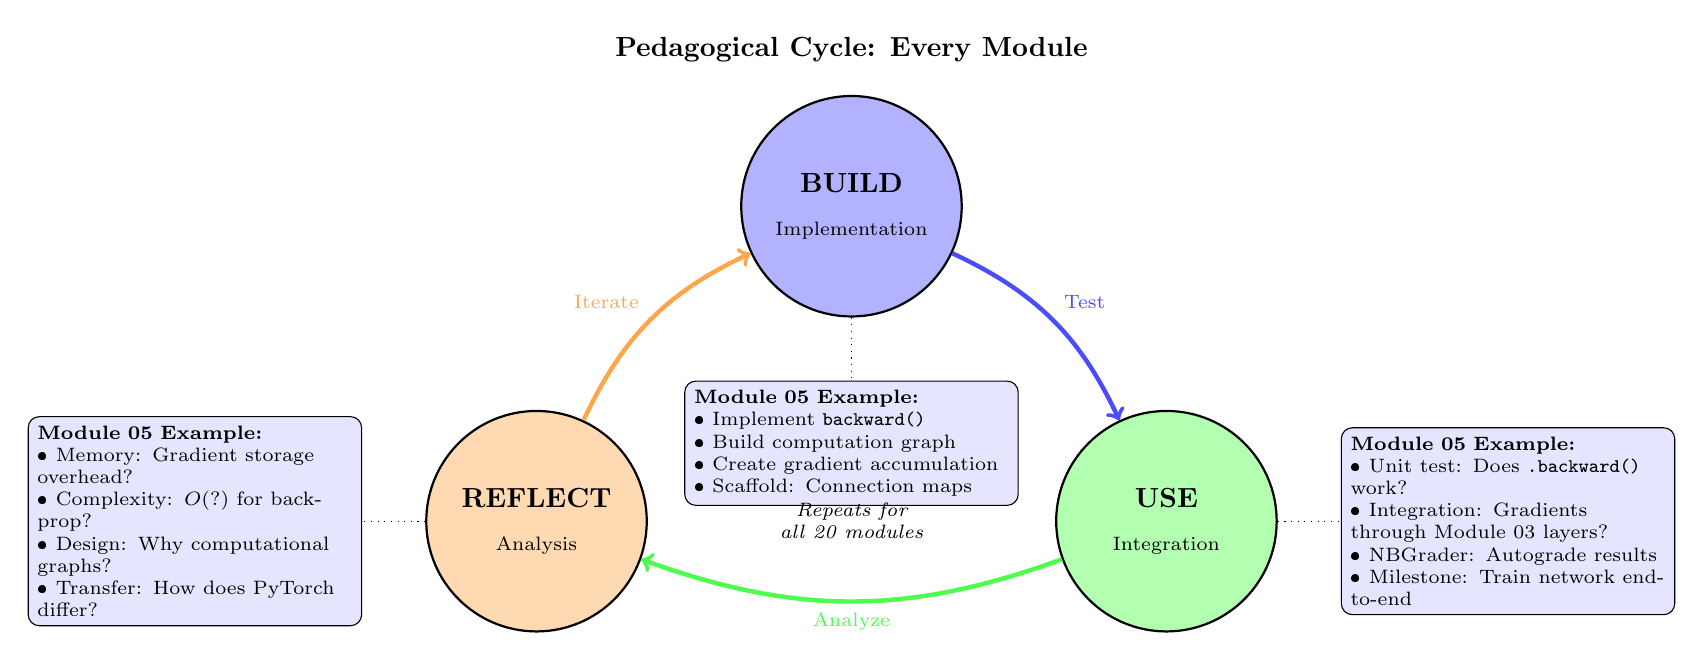
\begin{tikzpicture}[
    scale=1.0,
    every node/.style={font=\small},
    phase/.style={
        circle,
        draw,
        thick,
        minimum size=2.8cm,
        align=center,
        font=\normalsize\bfseries
    },
    example/.style={
        rectangle,
        draw,
        fill=blue!10,
        rounded corners,
        align=left,
        font=\scriptsize,
        text width=4cm
    }
]

% Three main phases in circular arrangement
\node[phase, fill=blue!30] (build) at (0, 4) {
    BUILD\\[0.3em]
    \normalfont\scriptsize Implementation
};

\node[phase, fill=green!30] (use) at (4, 0) {
    USE\\[0.3em]
    \normalfont\scriptsize Integration
};

\node[phase, fill=orange!30] (reflect) at (-4, 0) {
    REFLECT\\[0.3em]
    \normalfont\scriptsize Analysis
};

% Arrows connecting phases
\draw[->, ultra thick, blue!70] (build) to[bend left=20] node[midway, above right, font=\scriptsize] {Test} (use);
\draw[->, ultra thick, green!70] (use) to[bend left=20] node[midway, below, font=\scriptsize] {Analyze} (reflect);
\draw[->, ultra thick, orange!70] (reflect) to[bend left=20] node[midway, above left, font=\scriptsize] {Iterate} (build);

% Example boxes for each phase
\node[example, below=0.8cm of build] (build-ex) {
    \textbf{Module 05 Example:}\\
    • Implement \texttt{backward()}\\
    • Build computation graph\\
    • Create gradient accumulation\\
    • Scaffold: Connection maps
};

\node[example, right=0.8cm of use] (use-ex) {
    \textbf{Module 05 Example:}\\
    • Unit test: Does \texttt{.backward()} work?\\
    • Integration: Gradients through Module 03 layers?\\
    • NBGrader: Autograde results\\
    • Milestone: Train network end-to-end
};

\node[example, left=0.8cm of reflect] (reflect-ex) {
    \textbf{Module 05 Example:}\\
    • Memory: Gradient storage overhead?\\
    • Complexity: $O(?)$ for backprop?\\
    • Design: Why computational graphs?\\
    • Transfer: How does PyTorch differ?
};

% Connect examples to phases
\draw[dotted] (build) -- (build-ex);
\draw[dotted] (use) -- (use-ex);
\draw[dotted] (reflect) -- (reflect-ex);

% Center annotation
\node[align=center, font=\scriptsize\itshape] at (0, 0) {
    Repeats for\\
    all 20 modules
};

% Title annotation
\node[above=0.3cm of build, font=\normalsize\bfseries] {
    Pedagogical Cycle: Every Module
};

\end{tikzpicture}
\caption{Build→Use→Reflect pedagogical cycle structuring all TinyTorch modules. \textbf{Build:} Students implement components in Jupyter notebooks with scaffolded guidance (connection maps, TODOs). \textbf{Use:} Integration testing validates cross-module functionality via NBGrader unit tests and milestone checkpoints. \textbf{Reflect:} Systems analysis questions probe memory footprints, computational complexity, and design trade-offs. This cycle addresses cognitive apprenticeship by making expert thinking patterns explicit and assessment visible through automated feedback. Examples shown for Module 05 (Autograd).}
\label{fig:build-use-reflect}
\end{figure}

\clearpage

% ============================================================
% BONUS FIGURE: MILESTONE PROGRESSION
% ============================================================
\subsection*{Bonus Figure D: Historical Milestone Progression (MEDIUM PRIORITY)}
\textbf{Location:} Section 4.3 (Historical Validation), after milestone description\\
\textbf{Pedagogical Value:} Shows 70-year capability accumulation and which modules unlock each milestone.

\begin{figure}[h]
\centering
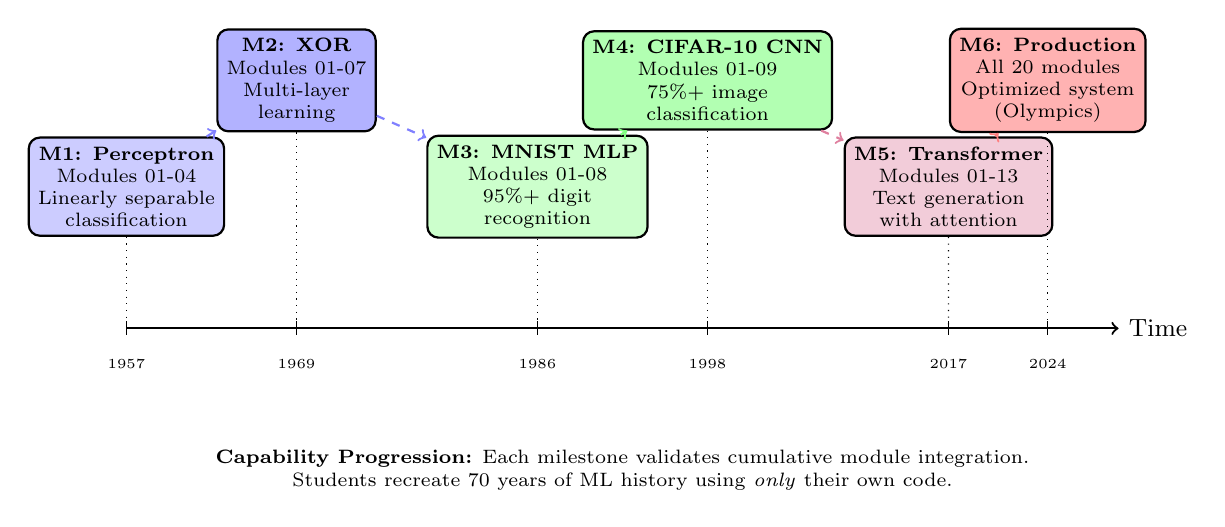
\begin{tikzpicture}[
    scale=0.9,
    every node/.style={font=\small},
    milestone/.style={
        rectangle,
        draw,
        thick,
        rounded corners,
        minimum width=2cm,
        minimum height=1.2cm,
        align=center,
        font=\scriptsize
    }
]

% Timeline axis
\draw[thick, ->] (0, 0) -- (14, 0) node[right] {Time};

% Year markers
\foreach \x/\year in {0/1957, 2.4/1969, 5.8/1986, 8.2/1998, 11.6/2017, 13/2024} {
    \draw (\x, 0.1) -- (\x, -0.1);
    \node[below, font=\tiny] at (\x, -0.3) {\year};
}

% Milestones
\node[milestone, fill=blue!20] (m1) at (0, 2) {
    \textbf{M1: Perceptron}\\
    Modules 01-04\\
    Linearly separable\\
    classification
};

\node[milestone, fill=blue!30] (m2) at (2.4, 3.5) {
    \textbf{M2: XOR}\\
    Modules 01-07\\
    Multi-layer\\
    learning
};

\node[milestone, fill=green!20] (m3) at (5.8, 2) {
    \textbf{M3: MNIST MLP}\\
    Modules 01-08\\
    95\%+ digit\\
    recognition
};

\node[milestone, fill=green!30] (m4) at (8.2, 3.5) {
    \textbf{M4: CIFAR-10 CNN}\\
    Modules 01-09\\
    75\%+ image\\
    classification
};

\node[milestone, fill=purple!20] (m5) at (11.6, 2) {
    \textbf{M5: Transformer}\\
    Modules 01-13\\
    Text generation\\
    with attention
};

\node[milestone, fill=red!30] (m6) at (13, 3.5) {
    \textbf{M6: Production}\\
    All 20 modules\\
    Optimized system\\
    (Olympics)
};

% Connect milestones to timeline
\foreach \m in {m1, m2, m3, m4, m5, m6} {
    \draw[dotted] (\m) -- (\m |- 0,0);
}

% Capability accumulation arrows
\draw[->, thick, blue!50, dashed] (m1) -- (m2);
\draw[->, thick, blue!50, dashed] (m2) -- (m3);
\draw[->, thick, green!50, dashed] (m3) -- (m4);
\draw[->, thick, purple!50, dashed] (m4) -- (m5);
\draw[->, thick, red!50, dashed] (m5) -- (m6);

% Accuracy progression annotation
\node[align=center, font=\scriptsize, fill=white] at (7, -2) {
    \textbf{Capability Progression:} Each milestone validates cumulative module integration.\\
    Students recreate 70 years of ML history using \emph{only} their own code.
};

\end{tikzpicture}
\caption{Historical milestone progression spanning 1957-2024. Each milestone requires progressively more modules, validating cumulative implementation correctness through historically significant achievements. Students experience ML's evolution from single-layer perceptrons (M1) through modern transformer architectures (M5) to production-optimized systems (M6). Arrows show capability accumulation - later milestones build on earlier foundations.}
\label{fig:milestone-progression}
\end{figure}

\end{document}
